\documentclass[border=10pt]{standalone}

\usepackage{tikz}
\usepackage{tikzsymbols}
\usetikzlibrary{calc,patterns,shapes.geometric}

\def\centerarc[#1](#2)(#3:#4:#5){\draw[#1] ($(#2)+({#5*cos(#3)},{#5*sin(#3)})$) arc (#3:#4:#5);}

\begin{document}
	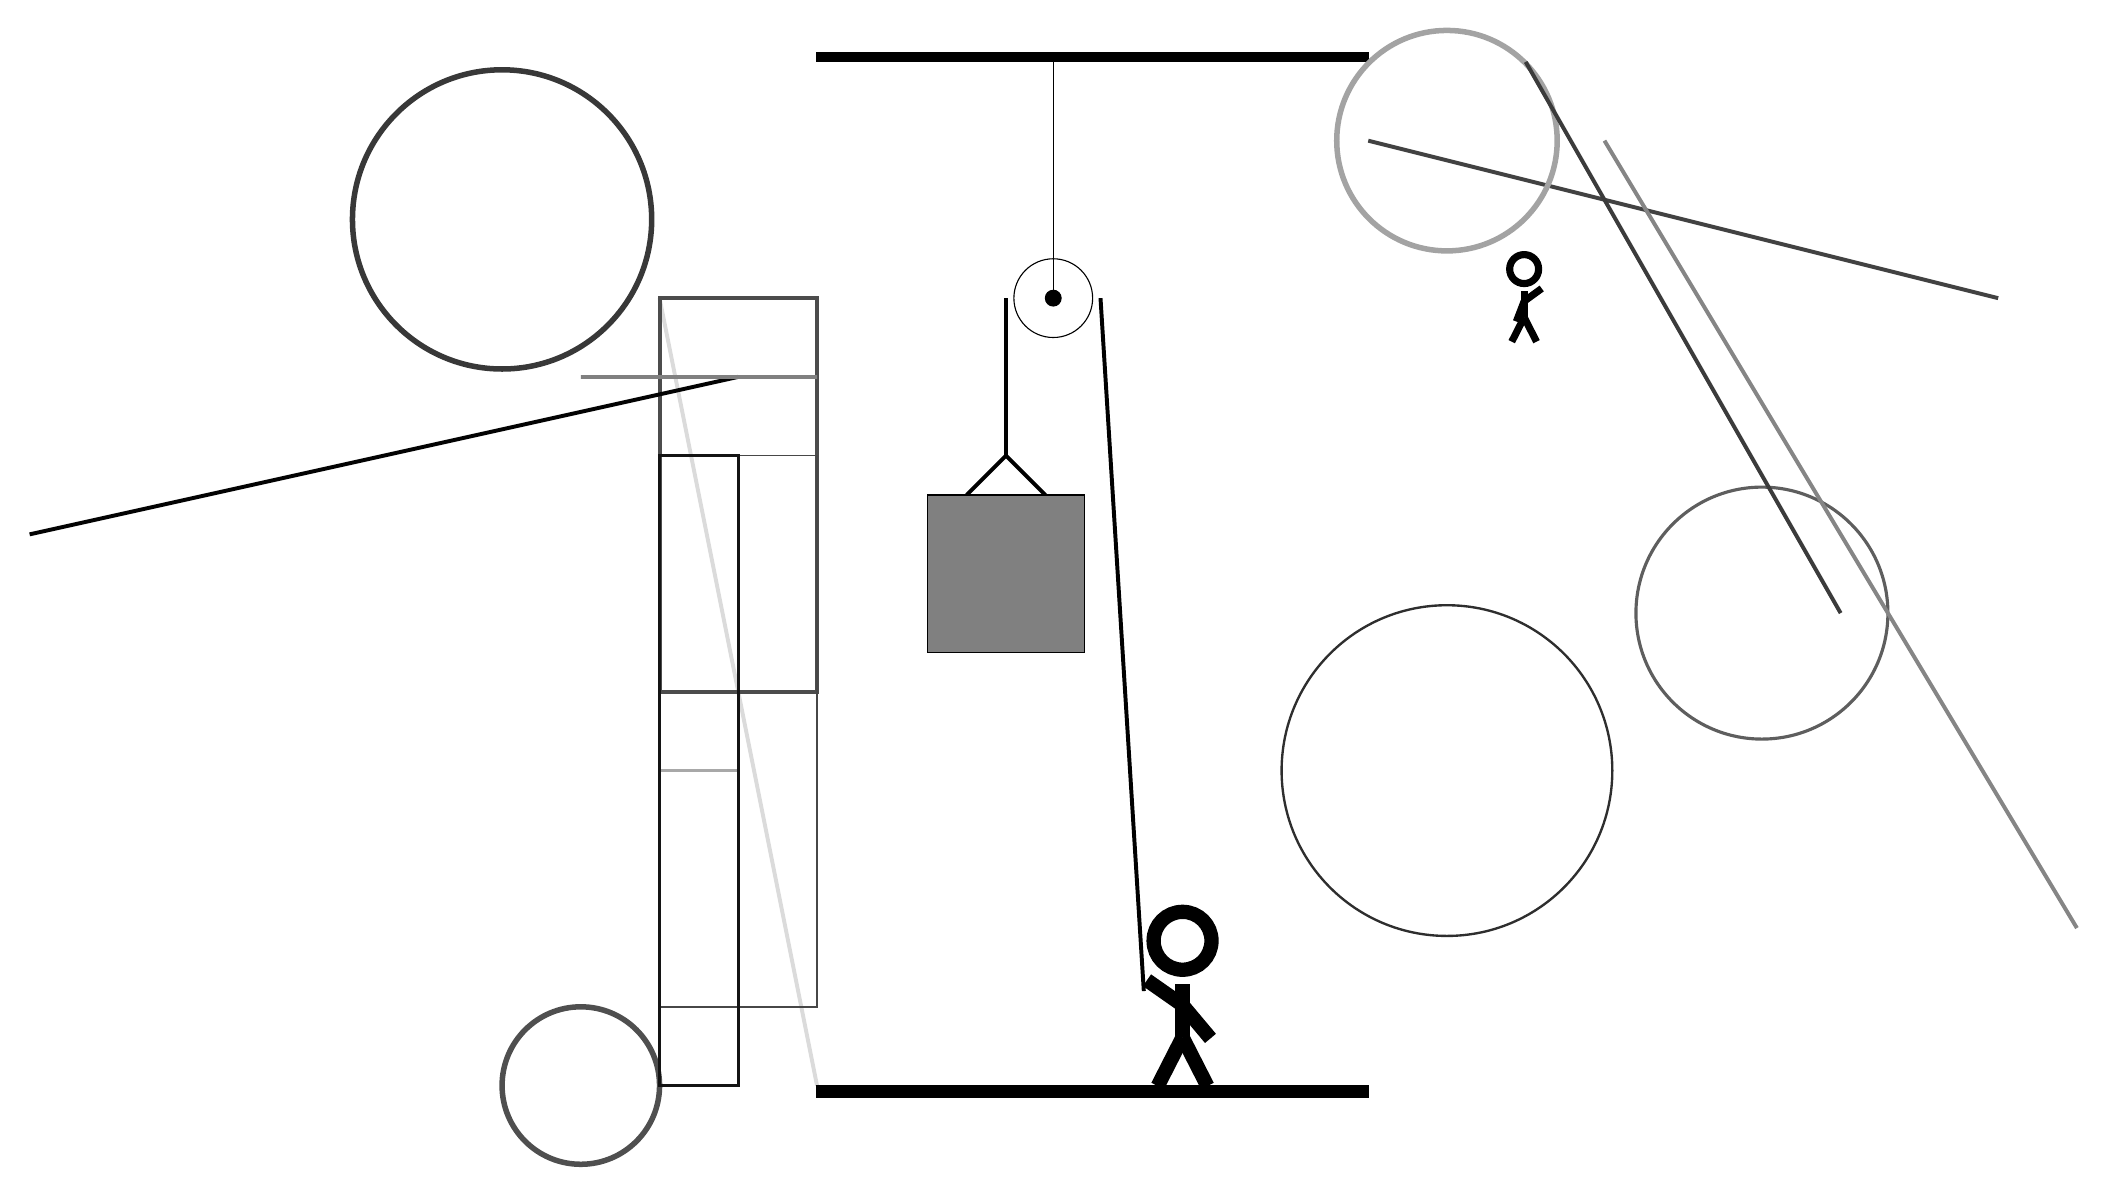
\begin{tikzpicture}
		%%%%% START %%%%%
		
		\draw[fill=black] (-2, 10) rectangle (5, 10.125);
		
		\draw (1, 7) circle (0.5);
		\draw[fill=black] (1, 7) circle (0.1);
		\draw (1, 10) -- (1, 7);
		
		\draw[line width=0.5mm, color=black!14](-4, 7) -- (-2, -3);
		
		\draw[line width=0.5mm, color=black!70] (-2, 7) rectangle (-4, 2);
		\node[line width=0.6mm, color=black!100] at (7, 7) {\Strichmaxerl[5][69][36]};
		\draw[line width=0.5mm, color=black!74](5, 9) -- (13, 7);
		
		\draw[line width=0.3mm, color=black!34] (-4, 1) rectangle (-3, -2);
		\draw [line width=0.7mm, color=black!36](6, 9) circle (1.4);
		\draw [line width=0.4mm, color=black!63](10, 3) circle (1.6);
		\draw[line width=0.5mm, color=black!99](-3, 6) -- (-12, 4);
		\draw[line width=0.2mm, color=black!72] (-2, -2) rectangle (-4, 5);
		\draw [line width=0.7mm, color=black!69](-5, -3) circle (1.0);
		
		\draw[line width=0.4mm, color=black!92] (-4, -3) rectangle (-3, 5);
		
		\draw[line width=0.5mm, color=black!48](8, 9) -- (14, -1);
		\draw[line width=0.5mm, color=black!77](7, 10) -- (11, 3);
		
		\draw [line width=0.7mm, color=black!78](-6, 8) circle (1.9);
		\draw [line width=0.3mm, color=black!82](6, 1) circle (2.1);
		\draw[line width=0.5mm, color=black!50] (-2, 6) rectangle (-5, 6);
		
		
		\draw[line width=0.5mm] (-0.1, 4.5) -- (0.4, 5.0) -- (0.9, 4.5);
		\draw[fill=black!50] (-0.6, 4.5) rectangle (1.4, 2.5);
		
		\draw[line width=0.5mm] (0.4, 7) -- (0.4, 5.0);
		\centerarc[line width=0.5mm](1, 7)(0:180:0.6);
		\draw[line width=0.5mm](1.6, 7) -- (2.15, -1.8);
		
		\node at (2.6, -1.9) {\Strichmaxerl[10][-35][-50]};
		
		\draw[fill=black] (-2, -3) rectangle (5, -3.15);
		
		%%%%% END %%%%%
	\end{tikzpicture}
\end{document}